\chapter{Analyse Fonctionnelle et Technique}
\label{chap:analyse_fonctionnelle}

\section{Analyse Fonctionnelle}

Pour comprendre l'objectif principal du projet nous avons réalisé une "bête à cornes" et un diagramme "pieuvre".

\subsection{Bête à cornes}
Le schéma "bête à cornes" permet d'expliquer simplement et facilement la mission du projet.
\begin{figure}[H]
    \centering
    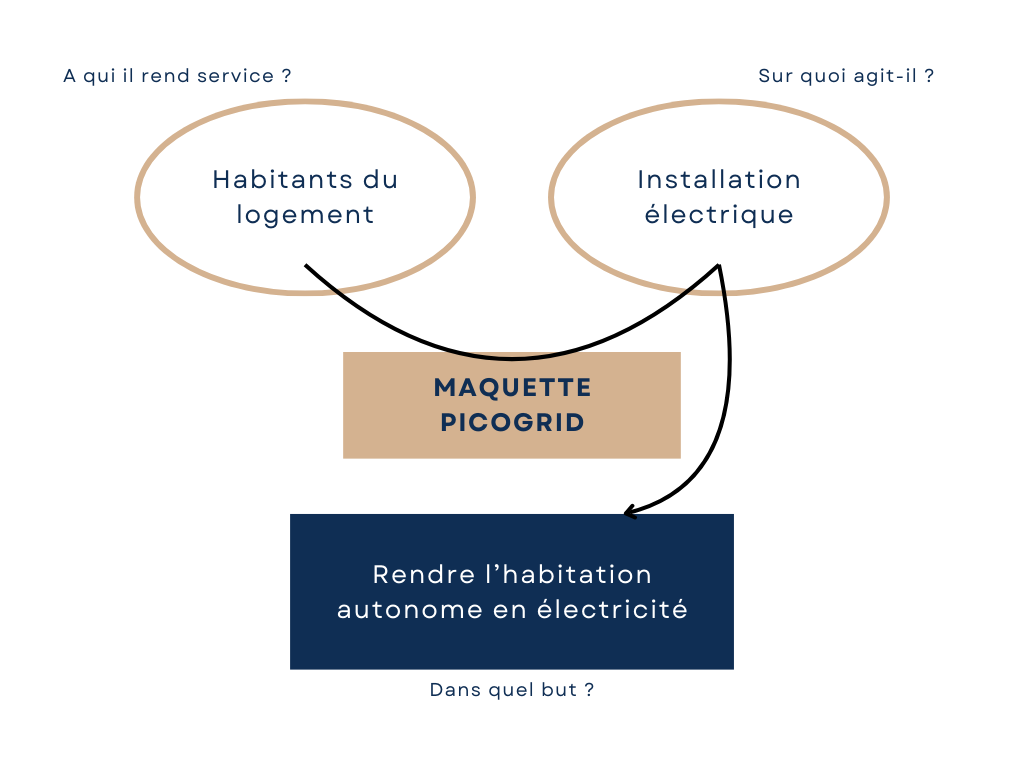
\includegraphics[width=0.8\textwidth]{images/diagrammes/Bête à cornes.png}
    \caption{Bête à cornes du projet}
    \label{fig:bete_a_cornes}
\end{figure}
Dans notre cas, la maquette Picogrid que nous allons réaliser est un dispositif conçu pour aider les habitants d'un logement à mieux gérer leur énergie. Son rôle est d'agir directement sur l'installation électrique de la maison afin de la rendre autonome. Ce système permet à l'habitation de produire et d'utiliser sa propre électricité, permettant son émancipation vis-à-vis du réseau électrique extérieur.

\subsection{Diagramme Pieuvre}
Le diagramme pieuvre permet de visualiser les fonctions de service du produit.
\begin{figure}[H]
    \centering
    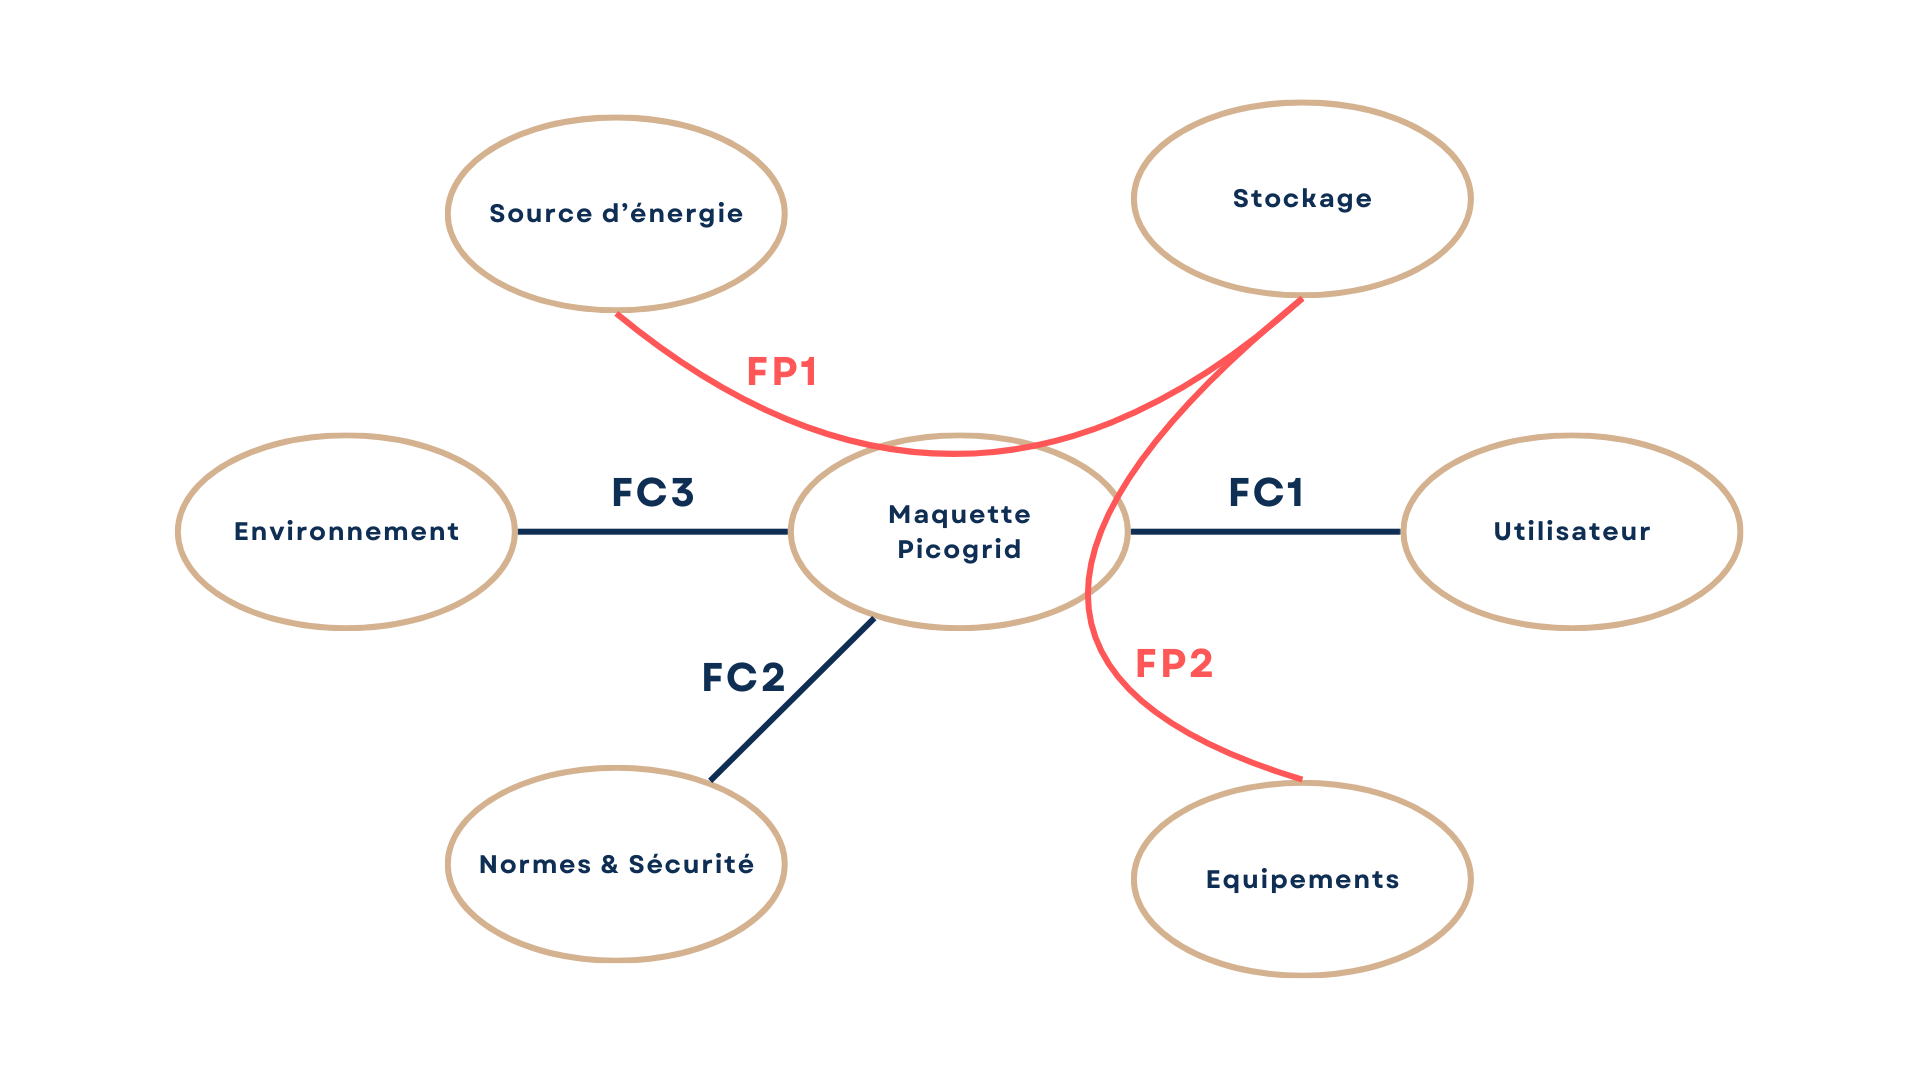
\includegraphics[width=0.8\textwidth]{images/diagrammes/Diagramme pieuvre.png}
    \caption{Diagramme Pieuvre du projet}
    \label{fig:pieuvre}
\end{figure}

\section{Rice Cooker}

\subsection{Caractéristiques Techniques du Rice Cooker}
\begin{itemize}
    \item \textbf{Puissance souhaitée} : 450\,W (contre 700\,W de base pour le fonctionnement normal du rice-cooker).
    \item \textbf{Nature de la charge} : Charge résistive et légèrement inductive. Une mesure réalisée au RLCmètre à 10\,kHz nous permet de trouver : $78\,\Omega$ et $10-11\,\mu H$.
    \item \textbf{Modulation} : L'alimentation doit être "modulable" pour faire varier la puissance de chauffe en fonction du mode désiré (cuisson et maintien en température).
    \item \textbf{Adaptation} : Fonctionnement en tension continue au lieu d'une tension alternative provenant du réseau (230\,Vac).
\end{itemize}

\subsection{Alimentation du Rice Cooker}
Le rice-cooker est un équipement qui permet de faire cuire du riz à l'aide d'une résistance qui va dissiper de la chaleur par effet Joule lors du passage d'un courant. C'est un équipement énergivore, donc on a limité sa puissance à 450\,W.

Son alimentation va nécessiter la création d'un convertisseur élévateur de tension continu (hacheur) avec les caractéristiques suivantes.

En supposant une tension d'entrée à 50\,V, on souhaite une puissance en sortie du convertisseur de 450\,W au maximum.

\subsubsection{Calcul du courant de sortie}
\begin{equation}
    I_s = \sqrt{\frac{P}{R}} = \sqrt{\frac{450}{78}} \approx 2,40\,\text{A}
\end{equation}
On en déduit la tension de sortie de notre convertisseur :
\begin{equation}
    V_s = \frac{P_s}{I_s} = \frac{450}{2,40} = 187,5\,\text{V}
\end{equation}

Donc le gain en tension de notre convertisseur devra être d'environ :
\begin{equation}
    G = \frac{V_s}{V_e} = \frac{187,5}{50} = 3,75
\end{equation}

Comme la puissance active est conservée (si on néglige les pertes dans le convertisseur), on obtient :
\begin{equation}
    P_s = P_e = 450\,\text{W}
\end{equation}
\begin{equation}
    I_e = \frac{V_s \times I_s}{V_e} = \frac{187,5 \times 2,40}{50} = 9\,\text{A}
\end{equation}

On aura donc un courant de 9\,A à l'entrée de notre convertisseur. Il faudra éventuellement prévoir un peu plus de puissance car il y aura des pertes dans le convertisseur. Les composants du hacheur ainsi que sa structure devront être choisis afin de respecter ces valeurs.

\subsection{Caractéristiques Techniques du Hacheur}
\begin{itemize}
    \item \textbf{Tension/courant d'entrée du convertisseur} : environ 50\,Vdc / 9\,A (voire un peu plus élevée quand les batteries sont chargées, batterie Plomb/Acide).
    \item \textbf{Tension/courant de sortie du convertisseur} : environ 187,5\,Vdc / 2,40\,A.
\end{itemize}

\section{Luminaires}

\subsection{Fonctions globales (Partie Puissance - Éclairage)}
\begin{itemize}
    \item Adapter la tension de la batterie (48\,V) aux besoins spécifiques du réseau d'éclairage.
    \item Distribuer l'énergie vers les 4 points d'éclairage LED définis (Cuisine, Salon, Coin lecture, Toilettes).
    \item Permettre l'allumage et l'extinction de chaque zone d'éclairage de manière manuelle et indépendante.
    \item Protéger matériellement les circuits d'éclairage contre les surintensités.
\end{itemize}

\subsection{Conversion d'énergie pour l'éclairage}
Le système doit être capable de transformer la tension continue issue de la batterie de stockage principale (plage de 42\,V à 56\,V) en une tension stable et sécurisée pour les luminaires de la maquette.

Pour cela nous devons mettre en place :
\begin{itemize}
    \item Un convertisseur DC/DC industriel du commerce abaissant la tension de la batterie (48\,V) vers un réseau 24\,V DC. Ce choix technologique présente un double avantage : il standardise le réseau secondaire avec les autres équipements de l'habitat (notamment le réfrigérateur), et il réduit significativement l'intensité du courant dans les câbles, minimisant ainsi les pertes par effet Joule.
\end{itemize}

Un dimensionnement optimisé pour une consommation totale inférieure à 20\,W, répartie de la manière suivante selon le besoin lumineux des pièces :
\begin{itemize}
    \item \textbf{Cuisine} : $\approx 6$\,W (Éclairage de travail fort)
    \item \textbf{Salon} : $\approx 5$\,W (Éclairage d'ambiance moyen)
    \item \textbf{Toilettes} : $\approx 3$\,W
    \item \textbf{Coin lecture} : $\approx 2$\,W (Éclairage minimal)
\end{itemize}
(Total estimé : $\approx 16$\,W, ce qui laisse une marge de sécurité technique pour le convertisseur).

\subsection{Distribution et commande de l'éclairage}
L'installation doit permettre un contrôle simple et direct par l'utilisateur. Ainsi le circuit de distribution doit comporter des interrupteurs mécaniques classiques sont placés sur chaque ligne pour contrôler les 4 zones séparément.

\section{Réfrigérateur}

\subsection{Fonctions globales (Partie Puissance - Réfrigération)}
\begin{itemize}
    \item Alimenter le réfrigérateur à partir du réseau de distribution continu adapté (24\,V).
    \item Assurer la production de froid de manière autonome.
\end{itemize}

\subsection{Caractéristiques de l'équipement}
D'après la plaque signalétique du réfrigérateur, les spécifications électriques requises sont :
\begin{itemize}
    \item \textbf{Tension d'entrée} : 12/24\,V d.c.
    \item \textbf{Puissance nominale} : 42\,W
\end{itemize}

\subsection{Tests et analyse de consommation}
Afin de valider le comportement électrique réel du compresseur sous 24\,V, nous avons effectué des mesures de courant :
\begin{itemize}
    \item \textbf{Régime transitoire (Démarrage)} : Lors de la mise en route, on relève un appel de courant générant un pic à 8\,A maximum.
    \item \textbf{Régime permanent} : Une fois la vitesse stabilisée, la consommation mesurée en continu s'établit à 1,4\,A.
\end{itemize}

\section{Distribution Ports USB}

\subsection{Fonctions globales (Partie Puissance)}
La partie distribution USB a pour objectif d'alimenter les équipements basse tension de l'installation à partir du bus batterie 48\,V.

Elle doit :
\begin{itemize}
    \item Adapter la tension 48\,V aux niveaux requis par les normes USB.
    \item Fournir une alimentation stable et sécurisée.
    \item Permettre la mesure de courant et tension pour le monitoring.
    \item Permettre le délestage en cas de batterie faible.
\end{itemize}

\subsection{USB-B (5V/2A)}
\subsubsection{Caractéristiques techniques}
La tension réelle du bus varie donc entre 42\,V et 56\,V, les convertisseurs DC-DC doivent être dimensionnés pour fonctionner sur toute cette plage.
\begin{itemize}
    \item \textbf{Tension de sortie} : 5\,V DC
    \item \textbf{Courant nominal minimal} : 2\,A (norme USB classique)
    \item \textbf{Puissance maximale estimée} : $P = 5\,\text{V} \times 2\,\text{A} = 10\,\text{W}$
\end{itemize}

\subsubsection{Conversion d'énergie}
La conversion 48\,V $\rightarrow$ 5\,V sera réalisée par un convertisseur DC-DC abaisseur (Buck synchrone).

\subsection{USB-C (20V/5A)}
\subsubsection{Caractéristiques techniques}
\begin{itemize}
    \item \textbf{Tension de sortie} : 20\,V DC
    \item \textbf{Courant maximal} : 5\,A
    \item \textbf{Puissance maximale} : 100\,W
\end{itemize}

\subsubsection{Conversion d'énergie}
La conversion 48\,V $\rightarrow$ 20\,V sera réalisée par un convertisseur DC-DC abaisseur.

\section{Monitoring}
Afin de pouvoir contrôler, monitorer et réguler l'ensemble de l'installation, il est fondamental de pouvoir mesurer avec précision les grandeurs électriques (tension et courant) à des points clés du circuit.

Ces données sont cruciales pour calculer la puissance produite par l'éolienne, la consommation de chaque équipement et l'état de charge de la batterie, permettant ainsi d'assurer le pilotage intelligent du système et le délestage des charges si nécessaire.

\subsection{Relevé des grandeurs électriques du système}
Le système doit être capable de connaître différentes valeurs de courant et tension en temps réel, et cela pour chaque équipement de l'installation électrique.
Pour cela nous devons mettre en place pour chaque convertisseur :
\begin{itemize}
    \item Un dispositif permettant de capter un niveau de courant;
    \item Un dispositif permettant de capter un niveau de tension.
\end{itemize}

Chaque convertisseur est associé à un dispositif de l'installation. Ainsi, nous aurons 6 convertisseurs pour les dispositifs suivants :
\begin{itemize}
    \item Frigo
    \item Rice cooker
    \item Éclairage
    \item USB-B
    \item USB-C
    \item Circuits électroniques
\end{itemize}

\subsection{Traitement et analyse des données}
Le système doit pouvoir traiter les données mesurées à chaque instant. Il doit être capable d'utiliser des valeurs de tension et courant pour déterminer des valeurs de :
\begin{itemize}
    \item La puissance générée par l'éolienne;
    \item La consommation de chaque équipement;
    \item L'état de charge de la batterie;
    \item Le temps restant estimé d'utilisation par équipement.
\end{itemize}

\subsection{Communication entre les dispositifs}
Les composants programmables (la Raspberry et les autres microcontrôleurs) présents dans le système doivent être en capacité de se transmettre des données. Il faut donc que chaque composant soit relié.